\section{Product architecture}
Our product consists of a plug-in developed for the Grafana platform and a Training Tool external to this platform. Therefore the analysis of the architecture is divided into these two components.

\subsection{Training tool}
The Training tool deals with training an SVM or LR algorithm using a dataset inserted by the user, to then generate a JSON file containing the necessary information to perform the prediction. This module has been developed following the \textit{MVVM} behavioural design pattern.

\subsubsection{Architectural design}
We decided to implement this pattern because React\glo was used to build the component and we believed that this pattern coupled well with the structure of the latter. Moreover, it allows to divide the \textit{Presentation Logic}\glo and the \textit{Business Logic}\glo and it allows to reuse some components in other contexts, without having to change them.

As can be seen in the following figure, we have the View that exchanges information on user interactions with the ViewModel, which in turn transforms them into actions on the data performed by the Model.
The data transition from the View to the Model occurs through the instantiation of the ViewModel inside the View. Through this instance, the ViewModel calls the correct functions when the user interacts with the View. The Model provides functionality for the management of the algorithms through the \texttt{SVMtrain} and \texttt{RLtrain} classes that will be used by the ViewModel. 
Finally there is a communication between Model and View for the constant updating of the latter, thanks to a functionality provided by the Grafana platform.

\begin{figure}[H]
\centering
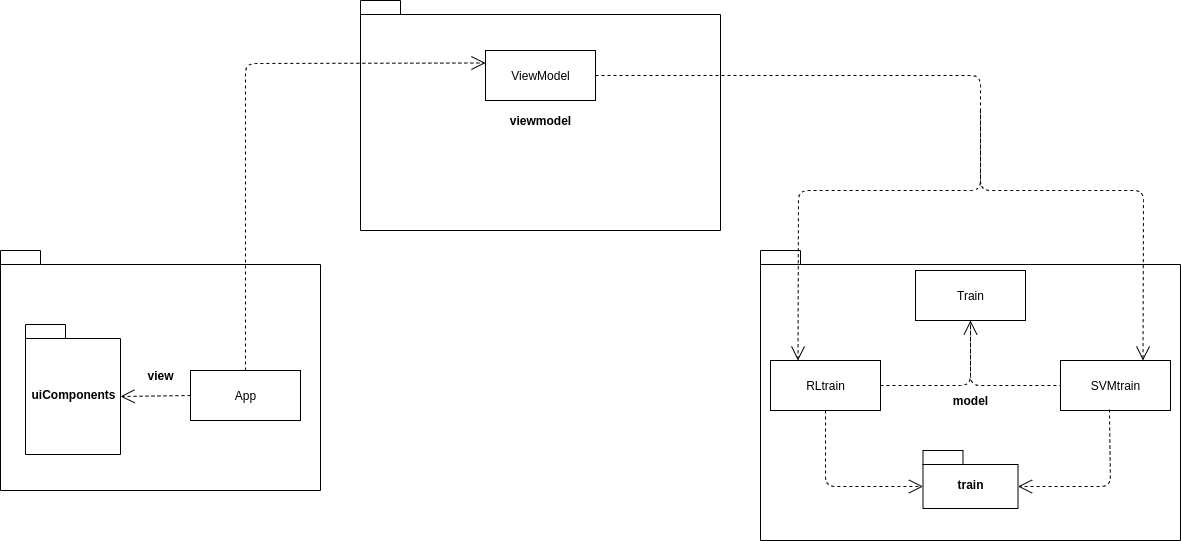
\includegraphics[scale=0.4]{../../../Diagrams/Package_diagrams/tool_design_patern.png}
\caption{Training tool package diagram}
\end{figure}

Analyzing the specific components, our architecture is structured as follows:
\begin{itemize}
\item \textbf{Model}: it manages the \textit{business logic}, in detail everything concerned the algorithms (such as libraries and their own methods);
\item \textbf{View}: it manages the \textit{presentation logic} through React, specifically what the user will see;
\item \textbf{ViewModel}: it manages the \textit{application logic}\glo. The ViewModel is an abstraction of the View exposing public commands, and  it has a binder, which automates communication between the View and its bound properties in the ViewModel.
\end{itemize}

\subsubsection{Detailed design}

\paragraph{Model}\mbox{} \\ \mbox{} \\
The main component of the Model is the abstract class of the prediction algorithms called Train. Starting with this, we have implemented two algorithms: Support Vector Machine and Linear Regression.
They are represented respectively by the concrete classes \texttt{SupportSVM}
and \texttt{SupportRL}. We have found that, for families algorithms such as Support Vector Machine and Linear Regression algorithms, it is possible to trace them to a single abstract class as we have provided. 

\paragraph*{SupportSVM}\mbox{} \\ \mbox{} \\
To implement the SVM algorithm we developed the concrete class \texttt{SupportSVM}. This class performs the prediction on the dataset. 
It also makes use of components specific to the SVM class imported from the SVM library to perform the real prediction. SupportSVM also has these fields data, each one instantiated by the constructor: \begin{itemize}
\item \texttt{dataSVM}: reference to the dataset;
\item \texttt{svm}: the SVM object;
\item \texttt{weights}: the weights are the SVM coefficients that will be used to make the prediction.
\end{itemize}
The constructor also defines the SVM options, such as the kernel (linear) and the karpathy (true). This class includes the method to perform the SVM train (\texttt{trainSVM()}) and the method to set the JSON file SVM structure up (\texttt{JSONData()}).


\paragraph*{SupportRL}\mbox{} \\ \mbox{} \\
To implement the Linear Regression algorithm we developed the concrete class \texttt{SupportRL}. This class performs the prediction on the dataset. It also makes use of components specific to the RL class imported from the RL library to perform the real prediction. SupportRL also contains these private fields data: \begin{itemize}
\item \texttt{dataRL}: reference to the dataset, instantiated by the constructor;
\item \texttt{numOfX}: the numbers of X founded on the CSV file;
\item \texttt{reg}: the RL object, which has 2 parameters: the X numbers (\texttt{dataRl.length}) and Y numbers (1);
\item \texttt{coefficients}: the coefficients needed to make the prediction, set as null by the constructor.
\end{itemize}
This class includes the method to perform the RL train (\texttt{trainRl()}) and the method to set the JSON file RL structure up (\texttt{JSONData()}).

\begin{figure}[H]
\centering
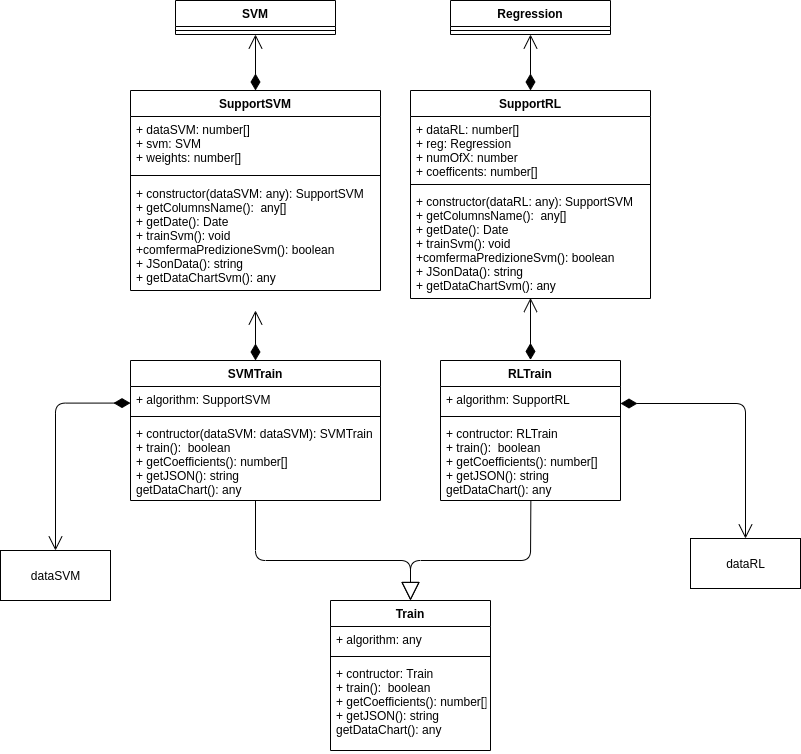
\includegraphics[scale=0.5]{../../../Diagrams/Classes_diagrams/tool_model.png}
\caption{Training tool Model class diagram}
\end{figure}

\paragraph{View}\mbox{} \\ \mbox{} \\
Inside the View there are all the view components.
The \texttt{App} class is the main component and it represents the tool's entry point. Each part of the View has been divided into components and rendered by the App. The communication between these components and the App takes place through the \texttt{props} (conceptually, the components are like JavaScript functions): it accepts arbitrary data (under the name of "props") and returns React elements that describe what should appear on the screen.
Inside there is an instance of the ViewModel for data-binding.

\subparagraph*{App}\mbox{} \\ \mbox{} \\
The \texttt{App} class is the main component and it represents the tool's entry point. Each part of the View has been divided into components and rendered by the App. This class has just one parameter: \texttt{viewModel} is an instance of the ViewModel. The constructor contains the properties in common with the ViewModel and the \texttt{viewModel} instance. Moreover, it has the following methods:
\begin{itemize}
\item \texttt{changeAlgorithm(event)}: it manages the algorithm user's choice, setting the \\ \texttt{algorithm} state value after the event was made;
\item \texttt{resetAlgorithm(algorithm)}: it sets the \texttt{algorithm} state parameter to the default value;
\item \texttt{setDataFromFile(data, fileInfo)}: it sets the \texttt{data} state parameter and the \\ \texttt{fileName} state parameter with the inserted file's name;
\item \texttt{handleTraining()}: it sends the data to the ViewModel and if the \texttt{performTraining()} method success, it calls the function to write the information into the JSON file, otherwise it resets the algorithm;
\item \texttt{downloadJsonData()}: it creates the DownloadJson component;
\item \texttt{render()}: it creates the InsertCsvButton, ComboBoxAlgorithm, TrainButton and Chart components and it calls the \texttt{downloadJsonData()} function;
\item \texttt{changeXAxis(event)}: it manages the xAxis user's choice to be displayed, setting the \texttt{xAixs} state value after the event was made;
\item \texttt{selectAxisX()}: if a file has been imported, it allows to change the X axis to be displayed;
\item \texttt{handleNotes(event)}: it manages the notes that have been written by the user, setting the \texttt{notes} state value after the event was made;
\item \texttt{handleName(event)}: it manages the file name that has been written by the user, setting the \texttt{changeName} state value after the event was made;
\item \texttt{show()}: it shows the "Information" page, which includes a step-by-step guide and the bugs report section;
\item \texttt{setDefaultName()}: if the new file name hasn't been written on the specific textArea, this method sets the default name of that file to: \textit{predictorsRL} if the CSV was a linear regression or \textit{predictorsSVM} if it was a SVM file.
\end{itemize}	

\subparagraph*{combo\_box\_algorithm}\mbox{} \\ \mbox{} \\
It renders the combo box for the algorithm's choice.\\
The \texttt{render()} method renders the JSX\glo element wanted.

\subparagraph*{download\_json}\mbox{} \\ \mbox{} \\
It manages and render the "Download" button.\\
The \texttt{downloadJsonFile()} method allow to download the file, making the connection between the browser and the local pc.
The \texttt{render()} method renders the "Download" button.

\subparagraph*{chart}\mbox{} \\ \mbox{} \\
It renders the chart.
This component contains the following parameters: 
\begin{itemize}
\item \texttt{data}: contains the data that must be shown;
\item \texttt{options}: contains the various options that can be applied to the graph, such as colors, axes and the regression line.
\end{itemize}
It also implements the following methods: 
\begin{itemize}
\item \texttt{formatData()}: it associates and manages the data to the graph;
\item \texttt{render()}: it renders the chart graph.

\end{itemize}

\subparagraph*{insert\_csv\_button}\mbox{} \\ \mbox{} \\
It renders the insert button for the CSV file.\\
The \texttt{render()} method renders the "Select file" button.

\subparagraph*{header}\mbox{} \\ \mbox{} \\
It renders the header.\\
The \texttt{render()} method renders the site's header.

\subparagraph*{train\_button}\mbox{} \\ \mbox{} \\
It renders the train button, that will start training.\\
The \texttt{render()} method renders the "Start training" button.

\subparagraph*{combo\_box\_x\_axis}\mbox{} \\ \mbox{} \\
It renders the combo box the axis's choice.
The \texttt{onChange} and \texttt{value} properties are \texttt{props} managed by the viewModel.

\subparagraph*{footer}\mbox{} \\ \mbox{} \\
It renders the footer of the page.

\subparagraph*{information}\mbox{} \\ \mbox{} \\
It renders the information page. It includes a brief guide for the tool and the email address to which bug reports should be sent.

\subparagraph*{textArea}\mbox{} \\ \mbox{} \\
It renders the textArea, which notes must be added to the JSON file produced.

\subparagraph*{textAreaFileName}\mbox{} \\ \mbox{} \\
It renders the textArea above the notes textArea, which information must be set as the JSON file name.

\begin{figure}[H]
\centering
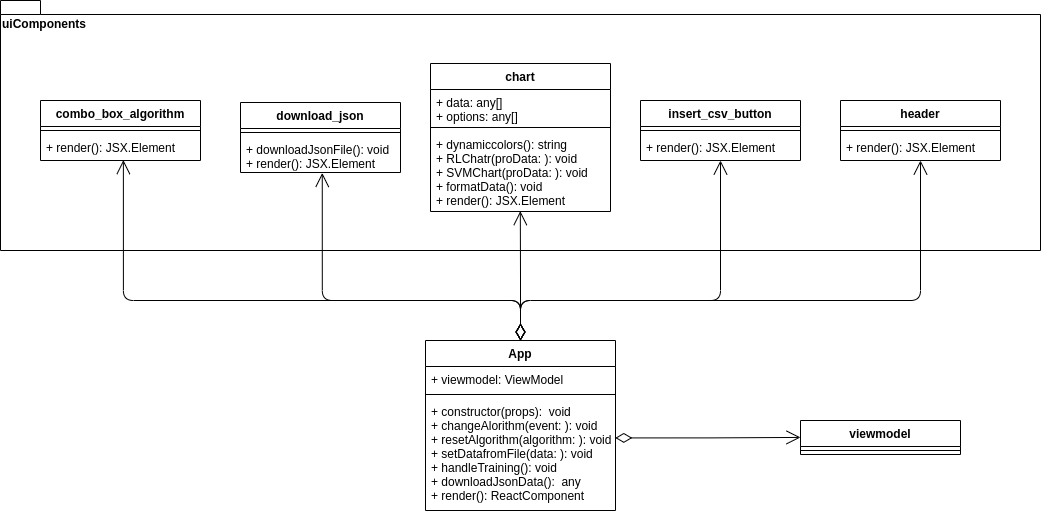
\includegraphics[scale=0.45]{../../../Diagrams/Classes_diagrams/tool_view.png}
\caption{Training tool Model class diagram}
\end{figure}

\paragraph{ViewModel}\mbox{} \\ \mbox{} \\
The data transition from the views to the model occurs through an instance of the ViewModel inside the View. Through this instance, the ViewModel calls the correct functions when the user interacts with the View.
The ViewModel has functions that interact with both the View and the Model (e.g. \texttt{RLChart()} and \texttt{performTraining()}).
To communicate with the Model, there is an \texttt{RLTrain} or \texttt{SVMTrain} instance. In order to instantiate the correct algorithm, the behavioural design pattern Strategy is applied. \\
The ViewModel contains the following private variables: \begin{itemize}
\item \texttt{algorithm}: it contains the string of the chosen algorithm (combo-box component);
\item \texttt{file}: it contains the data of the inserted CSV;
\item \texttt{hasFile}: true if the file CSV has been inserted, false otherwise;
\item \texttt{STrain}: it contains the strategy object;
\item \texttt{xAxis}: it contains the X axis of the CSV file;
\item \texttt{indexOfMax}: max index for the regression line to be displayed;
\item \texttt{indexOfMin}: min index for the regression line to be displayed;
\item \texttt{maxXAxis}: max X axis value;
\item \texttt{minXAxis}: min X axis value;
\item \texttt{notes}: it contains the notes that has been written on the textArea.
\end{itemize}
The \texttt{constructor()} set these variables to \texttt{null}.
Each variable has its own \texttt{set<<Variable>>()} function, that sets \texttt{this.<<Variable>>} to that variable. \\
The \texttt{checkAlgorithm()} method perform controls to the uploaded file: \begin{itemize}
\item if it is a SVM CSV file, the \texttt{verifyAlgorithm} calls the \texttt{isSVM} method;
\item if it is a RL CSV file, the \texttt{verifyAlgorithm} calls the \texttt{isRL} method;
\item if the CSV file does not match any prediction algorithm structure, the function returns an alert;
\item if any algorithm hasn't been chosen and we are trying to start training, the function returns an alert;
\item if the algorithm has been chosen but any file hasn't been inserted, the function returns an alert.
\end{itemize}
There are also the chart methods, that handle the datas to be displayed: \begin{itemize}
\item \texttt{straightLine()}: it uses the axis variables (xAxis, indexOfMax, indexOfMin, maxXAxis and minXAxis) to display the regression line correctly in the chart;
\item \texttt{chart()}: it sets the chart with the correct informations obtained by the uploaded file, in detail both X and Y axis;
\item \texttt{chartAxisX(label, dataX, dataY)}: it sets the color of the datas to be displayed: red if the data is "bad" (so miscalculated by the prediction algorithm) and green if the data is "good" (so correctly calculated);
\item \texttt{getPredictorsName()}: it returns the CSV columns names.
\end{itemize}

\begin{figure}[H]
\centering
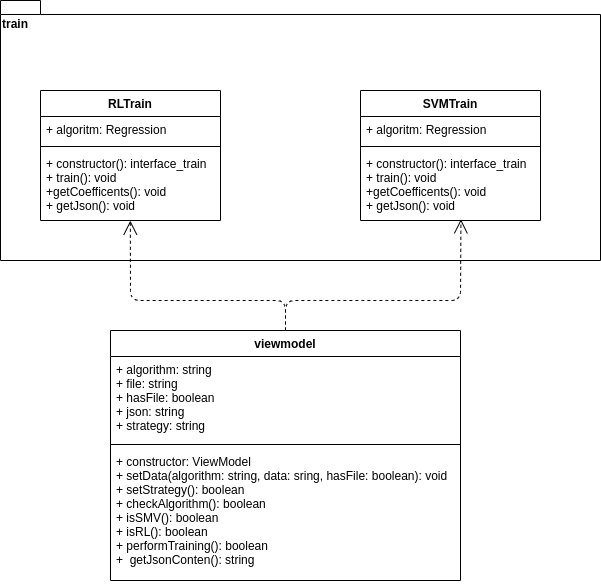
\includegraphics[scale=0.45]{../../../Diagrams/Classes_diagrams/tool_modelview.png}
\caption{Training tool Model class diagram}
\end{figure}

As it can be seen in this diagram, the ViewModel has a child class \texttt{StrategyTrain}, which is an implementation of the Strategy design pattern, that instantiate the correct algorithm whenever it's needed. Both \texttt{SVMTrain} and \texttt{RLTrain} classes are children of the \textit{abstract} \texttt{Train} class, so adding new algorithms in the future is simplified.

\paragraph*{SVMTrain}\mbox{} \\ \mbox{} \\
This class contains the methods to perform the SVM train, such as: \begin{itemize}
\item \texttt{train()}: it calls \texttt{algorithm.trainSvm()} to perform the train and it returns a boolean if the train has been done correctly (true) or it failed (false);
\item \texttt{getCoefficients()}: it gets the \texttt{algorithm.Weights()};
\item \texttt{getJSON()}: it gets the \texttt{algorithm.JSONData()}.
\end{itemize}
The constructor instantiate the private variable \texttt{algorithm} to a \texttt{new SupportSvm(dataSVM)} object.

\paragraph*{RLTrain}\mbox{} \\ \mbox{} \\
This class contains the methods to perform the RL train, such as: \begin{itemize}
\item \texttt{train()}: it calls \texttt{algorithm.insert()} to push the data and  \texttt{algorithm.trainRl()} to perform the train and it returns a boolean if the train has been done correctly (true) or it failed (false);
\item \texttt{getCoefficients()}: it gets the \texttt{algorithm.getCoefficientsRL()};
\item \texttt{getJSON()}: it gets the \texttt{algorithm.JSONData()}.
\end{itemize}
The constructor instantiate the private variable \texttt{algorithm} to a \texttt{new SupportRl(dataRl)} object.

\paragraph*{StrategyTrain}\mbox{} \\ \mbox{} \\
This class is the implementation of the Strategy design pattern, so it sets the strategy according to the CSV file inserted and the user's choice. \\
The constructor instantiates the \texttt{strategy} variable and the \texttt{data} variable to \texttt{null}. Therefore, the assignment of the strategy algorithm is deferred to method \texttt{setStrategy(algorithm, verifyAlgorithm}, which returns true if the strategy was set correctly or false if not. There are also the following methods: \begin{itemize}
\item \texttt{train()}: it calls the \texttt{train()} method of the specific strategy algorithm or it returns false;
\item \texttt{getJson()}: it calls the \texttt{getJson()} method of the specific strategy algorithm or it returns null;	
\item \texttt{getCoeff()} it calls the \texttt{getCoefficients()} method of the specific strategy algorithm;
\item \texttt{resetStrategy()}: it sets the \texttt{strategy} variable to \texttt{null};
\item \texttt{hasStrategySet()}: it return true if the \texttt{strategy} is not null, false if not;
\item \texttt{setData()}: it sets the private variable \texttt{data} to the specific \texttt{data}, which will be used for the prediction.
\end{itemize}

\paragraph*{abstractTrain}\mbox{} \\ \mbox{} \\
The base class, useful to add new prediction algorithms in the future. \\
It represents the contract that all concrete classes must abide to be able to characterize a prediction algorithm. It contains only one parameter: \texttt{algorithm}, set to \texttt{null}.

\paragraph*{Sequence diagram}\mbox{} \\ \mbox{} \\
To better explain the set of actions performed in order to process the data for
predict algorithms, the following picture illustrate a sequence diagram which examines SVM. The procedure is also indicative for the others algorithms.

\begin{landscape}
\begin{center}
\begin{figure}[H]
\centering
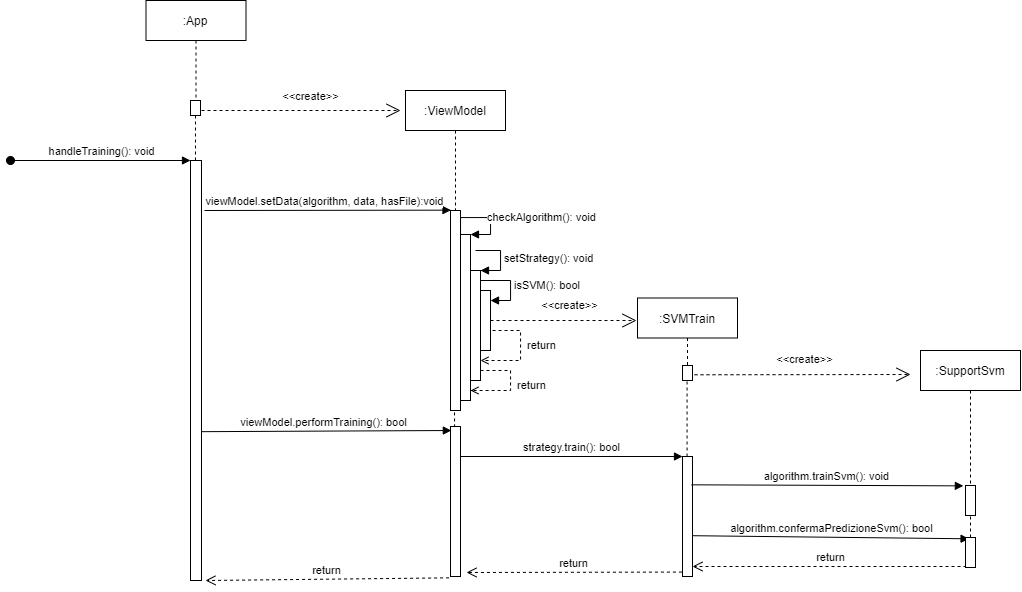
\includegraphics[scale=0.60]{../../../Diagrams/Sequence_diagrams/trainSVM.png}
\caption{TrainSVM sequence diagram}
\end{figure}
\end{center}
\end{landscape}

\subsection{Prediction plug-in}
The Prediction Plug-in will take care of receiving the json input and once the predictors have been connected to a data flow, will allow you to start making calculations forecasting. This module has been developed following the \textit{MVC} design pattern.

\subsubsection{Architectural design}
We felt that this model coupled well with the Grafana plug-in structure.
Moreover, it allows to divide the \textit{presentation logic} and the \textit{business logic} and it allows to reuse some components in other contexts, without having to change them (e.g. the View).
In this module, consisting of several panels within Grafana, the predictor, produced by the external tool, will be associated with the data flow monitored in Grafana. For this module the \textit{MVC} architectural pattern was used. In this architecture the \texttt{Editor} and the \texttt{Panel} share the variable \texttt{props}, instantiated by Grafana.

\begin{figure}[H]
\centering
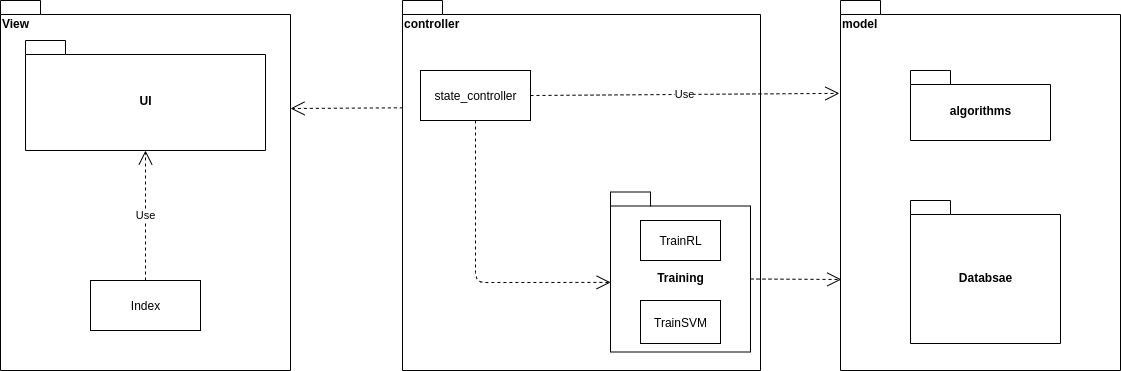
\includegraphics[scale=0.45]{../../../Diagrams/Package_diagrams/plugin_design_pattern.png}
\caption{Prediction plug-in package diagram}
\end{figure}

Analyzing the specific components, our architecture is structured as follows:
\begin{itemize}
\item \textbf{Model}: it manages the \textit{business logic}. It contains
the data prediction algorithms that have been presently implemented and writing the result of the predictions to an Influx database;
\item \textbf{View}: it manages the \textit{presentation logic}. It allows the creation of a customized graphic panel within a Grafana dashboard. With this panel the user can select prediction algorithm settings, incoming data streams and the minimum and maximum thresholds;
\item \textbf{Controller}: it manages the \textit{application logic}. It transforms the data obtained from user interactions and data flows obtained by Grafana in a format suitable for carrying out the actions by the Model.
\end{itemize}


\paragraph{Grafana's role}\mbox{} \\ \mbox{} \\
Grafana plays a fundamental role in the architecture as it allows continuous updating of the View to change the data in the Model. In particular, whenever there are updates on the data in the Model, Grafana makes them available to View through specific methods, together with the configuration of the queries with which this data was obtained. Moreover, through React, it manages the two-way data binding between HTML View and Javascript code, in addition to offering most of the necessary graphic components for the realization of the plug-in View.

\subsubsection{Detailed design}
\paragraph{Model}\mbox{} \\ \mbox{} \\
The Model is the implementation of the \textit{Strategy} pattern. Unlike the tool, in this case the pattern is used to implement the forecast calculation algorithms.
The algorithms are instantiated by the Controller when a JSON file containing the definition of the algorithm to be used is read, therefore extrapolating the values to be passed to the constructors always from the file just inserted.\\
The Model's main component is the interface of the prediction algorithms
called \texttt{Algorithm}. Starting with this, we have implemented
two algorithms: Support Vector Machine and Linear Regression.
They are represented respectively by the concrete classes Svm and Regression. We have found that, for families of Support Vector Machine and Regression algorithms, it is possible to trace them to a single interface as we have provided.

\paragraph*{Algorithm}\mbox{} \\ \mbox{} \\
The interface of the prediction algorithms is called \textit{Algorithm} and it
represents the contract that all concrete classes must abide by
to be able to characterize a prediction algorithm. It contains only one method:
\texttt{predict(input)}. This allows you to perform the prediction on a specific dataset of type \texttt{number}.

\paragraph*{Influx}\mbox{} \\ \mbox{} \\
This class is used to interface and write data to the Influx database WriteInflux. \texttt{InfluxDB} contains an instance of the Influx DB and the \texttt{write()} method writes the data to the Influx database. The async method \texttt{connect(host, port, database, username?, password?)} it's used to connect the database to the plug-in. Any other "connection-handling method", \texttt{setMeasurement} and \texttt{setDatasource} methods are handled by the \textit{controller}.

\begin{figure}[H]
\centering
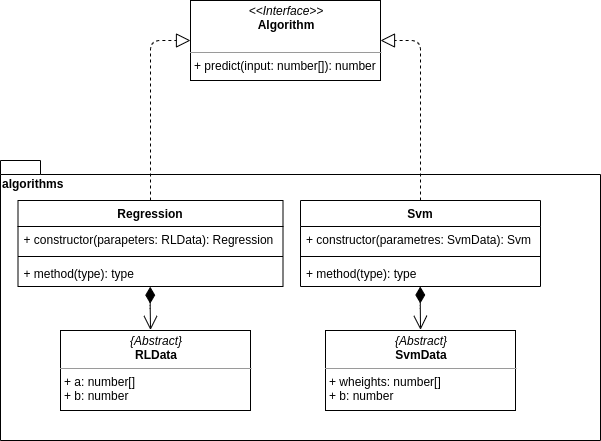
\includegraphics[scale=0.40]{../../../Diagrams/Classes_diagrams/plugin_model.png}
\caption{Prediction plug-in Model class diagram}
\end{figure}

\paragraph{View}\mbox{} \\ \mbox{} \\
The main node of the View is the \texttt{Editor} class, which is the composition of different graphic objects such as CollegamentoView, PrevisioneView, ListaCollegamentiView and CaricamentoJsonView. The latter correspond to the panels and internal objects that will be shown by the plug-in. \\
All these classes are subclasses that extend the React class \texttt{React.PureComponent} which allows you to create components in React:
\begin{itemize}
\item \texttt{CaricamentoJsonView}: it is a view that takes care of loading the JSON file containing the definition of the algorithm previously trained by the training tool;
\item \texttt{CollegamentoView}: this view allows the user to insert a new link, connect a data flow node to the latter and set the thresholds;
\item \texttt{ListaCollegamentiView}: this view lets the user to modify or delete the previous links created;
\item \texttt{PrevisioneView}: this view allows the user to start or stop the monitoring and save the prediction on the Influx database.
\end{itemize}
The \textit{Observer} pattern was used to simplify communication between the Controller and the View components that need to be updated as a result of changing the state of the Controller. In our case the subject class, when it undergoes a status change, it notifies the other components via the \texttt{update()} method.

\begin{figure}[H]
\centering
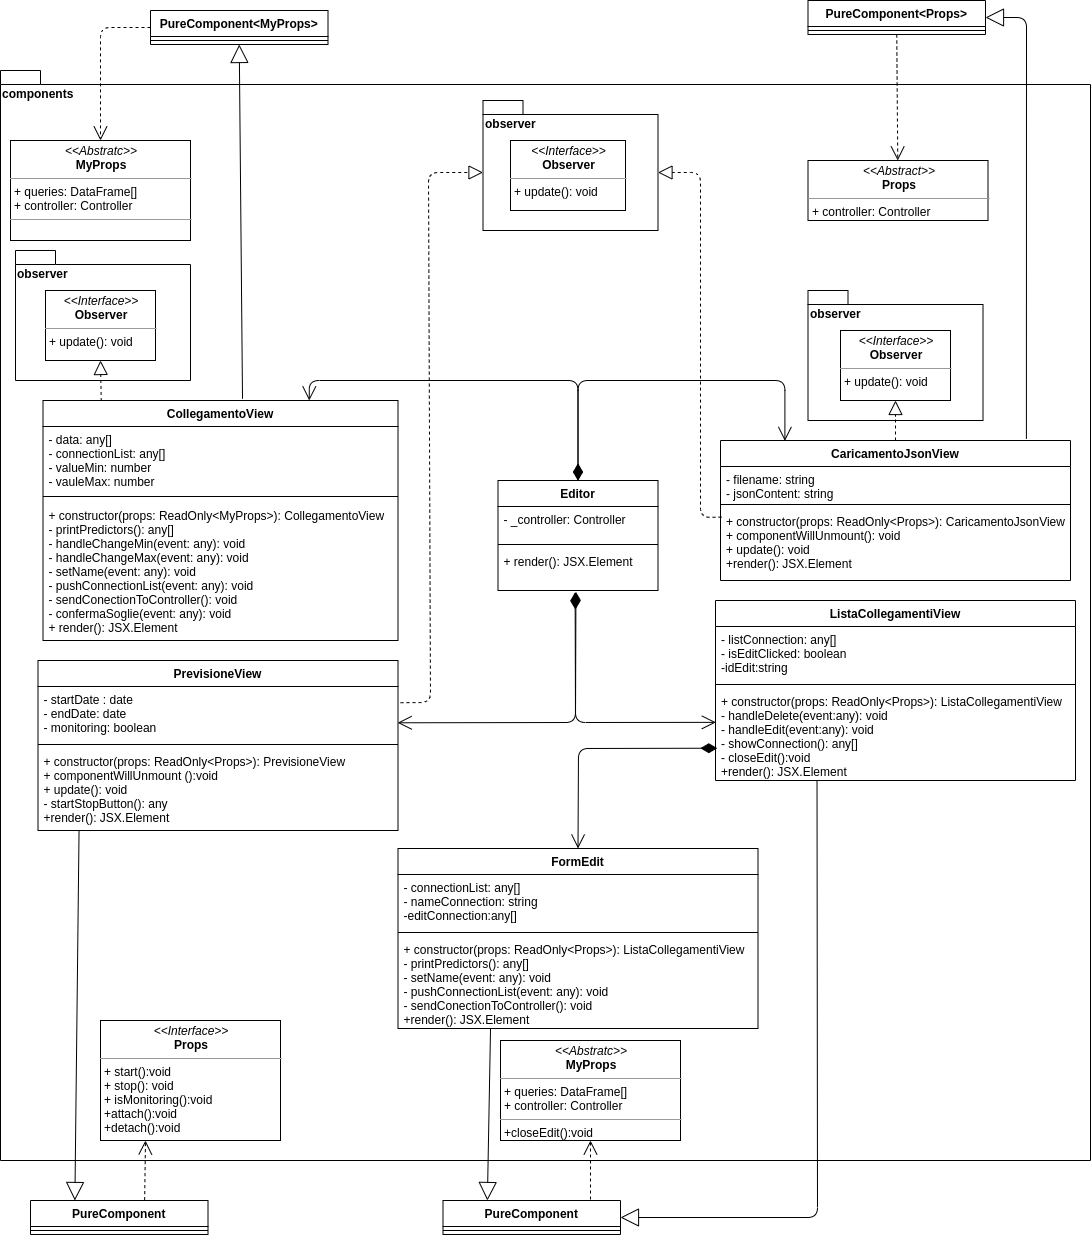
\includegraphics[scale=0.40]{../../../Diagrams/Classes_diagrams/plugin_view.png}
\caption{Prediction plug-in View class diagram}
\end{figure}

\paragraph{Controller}\mbox{} \\ \mbox{} \\
The controller implements the \textit{Observer} pattern; in this case the controller class extends the abstract observable class which therefore represents the subject to be observed, the observer will instead be the view classes.
The Controller will notify the views whenever it changes its state, particularly when the JSON file is inserted and read and when the monitoring is started or stopped.\\
When importing the JSON file, the controller will take care of: \begin{itemize}
\item read its contents through the \texttt{setJson(file)} function. Once the Controller finishes reading the file, it notifies the View via the \texttt{update()} method, showing the new information obtained from the file;
\item save a copy of the predictors;
\item apply the correct forecasting algorithm through the \texttt{setStrategy()} method;
\item notify the JSON file upload success views.
\end{itemize}
Moreover, it manages the database functions, which allow to add, edit or remove a connection, set new measurements, update and set datasources and save predictions on the Influx database.\\

\begin{figure}[H]
\centering
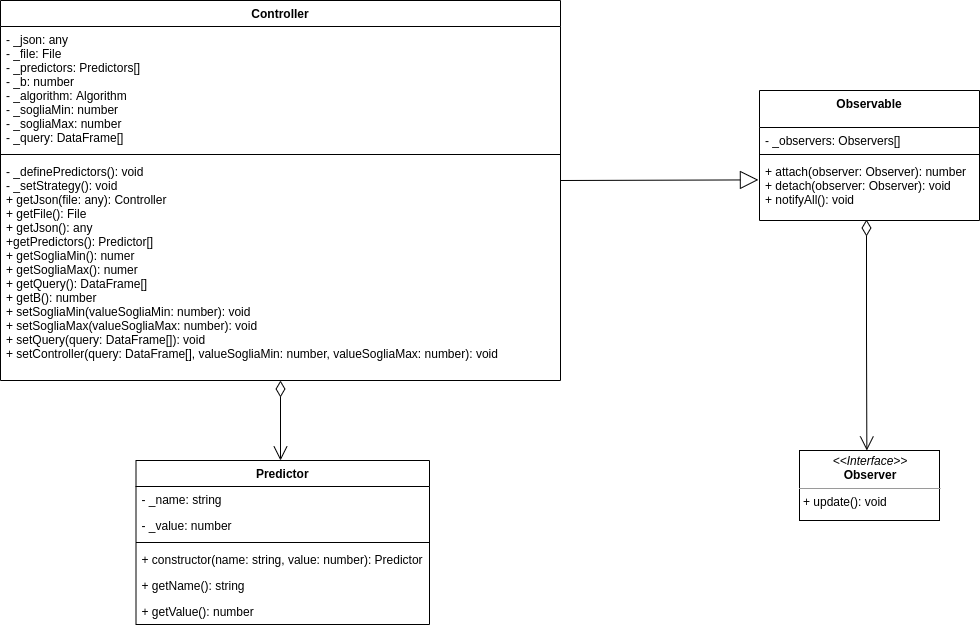
\includegraphics[scale=0.40]{../../../Diagrams/Classes_diagrams/plugin_controller.png}
\caption{Prediction plug-in Controller class diagram}
\end{figure}

\paragraph*{Sequence diagram}\mbox{} \\ \mbox{} \\
The following sequence diagram describes the \texttt{viewGraph()} method, that 
process the data and updates the Grafana's graph with the correct algorithm prediction.

\begin{center}
\begin{figure}[H]
\centering
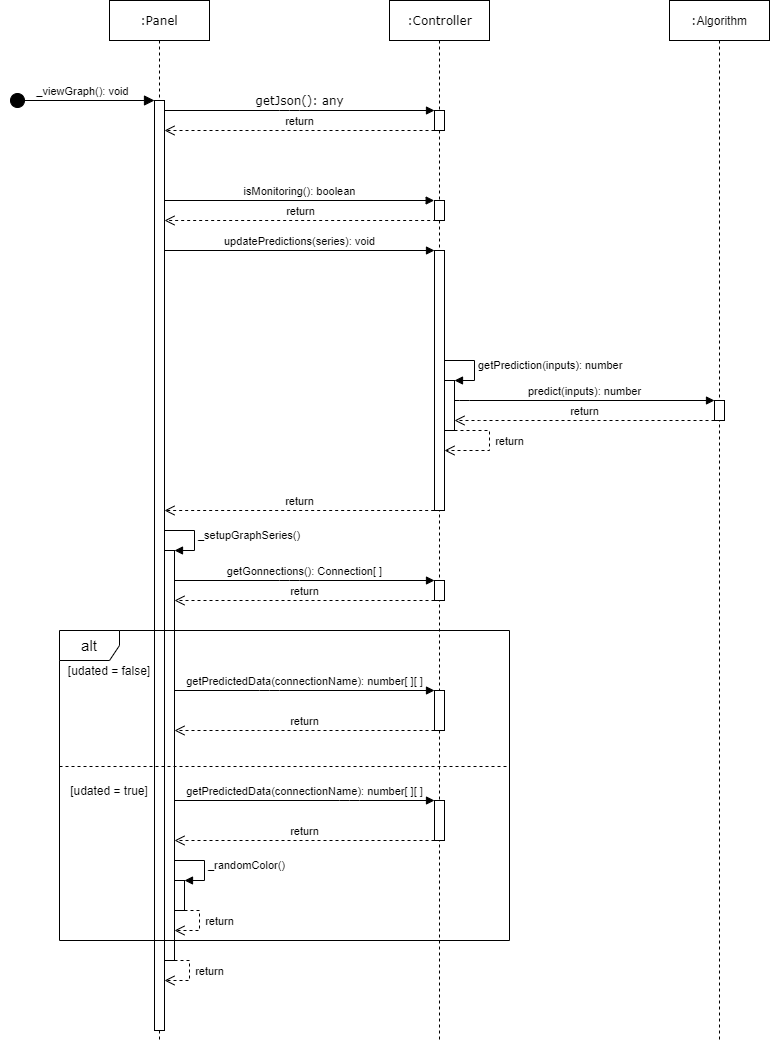
\includegraphics[scale=0.55]{../../../Diagrams/Sequence_diagrams/viewGraph.png}
\caption{\texttt{viewGraph()} sequence diagram}
\end{figure}
\end{center}